\chapter{Introduction}


\section{Cosmology and the cosmic dawn}

\subsection{Modern cosmology and the history of the universe}

Much like particle physics, cosmology today finds itself in the enviable yet frustrating position of having a broadly supported picture of the universe with only the most challenging and fundamental questions unanswered. Many intersecting lines of evidence point to a universe which began hot, dense, homogenous, and rapidly expanding 13.8 billion years ago, eventually cooled enough for bound objects to form, and is now accelerating. Studies of the Cosmic Microwave Background (CMB), high-z supernovae, distant galaxies, primordial element abundances, the matter power spectrum, and other observables all converge on this model. It is largely, however, a mal-understood and entirely unexpected \textit{dark} universe, whose total energy budget is dominated by constituents whose gravitational properties are well understood, but whose fundamental nature remains mysterious. 

The simplest (i.e., \textit{vanilla}) model which agrees with all available data is parameterized by the energy densities of baryons ($\Omega_b=0.0455\pm0.0003$), cold dark matter  ($\Omega_m=0.3089\pm0.0062$), and vacuum energy ($\Omega_\Lambda=0.69\pm0.0062$), the amplitude ($\ln (10^{10}A_s)=3.064\pm0.023$) and spectral index ($n_s=0.9667\pm0.004$) of the primordial power spectrum, and the optical depth to reionization ($0.066\pm0.012$). 
The energy densities are given as the present densities of these constituents relative to the present critical density $\rho_c=3H_0^2/8\pi G$, where the present expansion rate is $(70\pm3$)\,km/s/Mpc
\footnote{I've taken the uncertainty on $H_0$ to be the spread between the CMB measurement of $67.74\pm0.46$ km/s/Mpc \citep{planck16} and the local measurement of $73.2\pm1.7$ \citep{reiss16}.}. 
On scales larger than hundreds of Mpc, our universe is flat, deviating from Euclidian geometry only due to a homogenous and isotropic expansion, with a measured curvature density consistent with zero of $\Omega_K=0.008\pm0.004$. 
Further, the equation of state of dark energy is constrained to be $w=-1.02\pm0.08$, consistent with -1, and thus, with a true cosmological constant or a uniform vacuum energy. These measurements represent the best combined constraints reported by \citet{planck16}, and have been made possible by the avalanche of data on the CMB, weak lensing statistics, baryon acoustic oscillations, and type 1a supernova surveys collected in recent years. 

In this framework, the history of the universe is fairly well established. Nuclear reactions in the first few minutes of the universe created Hydrogen, Helium, Lithium, and trace amounts of deuterium and lithium, and astronomers have verified these predictions of primordial abundances to high precision \citep{bbn}. After 370,000 years of expansion and cooling, the photon mean free path increased to larger than the Hubble radius and protons and neutrons formed atoms. The CMB is that relic photon gas, and its anisotropies represent order $10^-5$ density and temperature fluctuations at recombination. After the release of the CMB, before sources formed, those slight fluctuations began to collapse under gravity during a period known as the dark ages. After a few hundred million years, sufficient densities and temperatures were reached in these collapsing halos to form the first bright sources in a period known as the cosmic dawn, culminating in the epoch of reionization. 

The basic sequence of events is well understood. These very massive and bright stars (known as Population III stars) formed from primordial (metal-free\footnote{Note that in astronomy nomenclature, all atoms heavier than Helium are known as \text{metals}.}) gas are thought to have irradiated the IGM with ionizing photons, reionizing the formerly neutral intergalactic medium. Nucleosynthesis processes in their supernova are thought to have polluted galaxies with the metals needed for gas to more easily collapse and cool, allowing modern stars to form. 

Many questions remain about this first generation of sources. How massive were they? How bright? How numerous? What were the relative contributions of stars, black hole binaries, and quasars? When exactly did these first stars form and how long did it take? How many linger in stellar halos? Simple n-body simulations can model the gravitational collapse of the cosmic web and dark matter halos, but complex feedback and subgrid physics models are needed to understand the the baryonic processes involved in the formation of stars and galaxies. It is no wonder progress has been slow, these stars and galaxies are by definition the farthest and faintest ones that can ever hope to observe, and understanding their formation, before any stars even shone at all, is even more of a challenge. 

This thesis presents experimental work in the field of 21\,cm cosmology, a promising avenue to circumvent the catch-22 of how to study galaxies before they began to emit light. The idea, which I discuss in detail in Sec. \ref{sec:intro21cmsection}, is to study not the galaxies themselves, but instead the intergalactic medium between them. In particular, we seek to measure the slight low frequency radio emission from the neutral hydrogen between galaxies in order to map out the matter distribution of the universe, and then once stars begin to form and irradiate this neutral gas, observe the resulting ionized bubbles growing around galaxies over cosmic time. 

Eventually the whole volume of the intergalactic medium is ionized, and this last phase transition of the universe is known as the Epoch of Reionization, thought to have occurred in the first few hundred million years of the universe ($6\lesssim z\lesssim12$), following the Dark Ages ($20\lesssim z\lesssim 1100$) when gravitational collapse assembled the galaxies themselves. Broadly, the study of the formation and evolution of these first stars and galaxies is known as the Cosmic Dawn, and it is the missing link between the hot, smooth post-big bang universe and the modern clumpy universe we know today.


\subsection{Reaching towards the cosmic dawn}

For all the questions about the astrophysics of reionization and the lack of direct observations, a number of indirect constraints establish a rough picture of the EOR and bound its beginning and end. 

% Ly-alpha forest
The Lyman alpha forest and its transformation into Gunn-Peterson trough at $z\sim6$ provide perhaps the clearest evidence of the evolving ionized fraction of the IGM. Quasars are an observational category of active galaxies whose smooth spectrum jets happen to be oriented along our line of sight. At redshifts $1<z<3$ the band between Lyman continuum and Lyman alpha becomes increasingly crowded with absorption lines, indicating that these quasar beams have traversed more and more neutral hydrogen clouds at intermediate redshifts. Between $3<z<5$, these lines become so crowded, that there is no apparent continuum level, and at higher redshifts close to the end of reionization, there are enough neutral hydrogen atoms left everywhere that all emission in this band is absorbed. A caveat is that the Lyman alpha line saturates at even very small neutral fractions down to $\sim10^{-5}$ \citep{FurlanettoReview}, so the appearance of a Gunn-Peterson trough is evidence only of the tail end of reionization. The mid point and indeed the whole reionization history is unconstrained by these observations.

SHOW THE GRAPHIC THAT TOM IS MAKING FOR ME

% CMB optical depth measurements
An orthogonal constraint on the redshift of reionization derives from the measurement of the thompson scattering optical depth $\tau$ between us and recombination. Scattering of CMB photons off free electrons tends to smear out the temperature anisotropies, damping the power on all angular scales scales as $e^{-2\tau}$, however there are no free electrons in the intergalactic medium immediately after recombination. Such scattering does not occur until the epoch of reionization, when the first sources irradiate the neutral IGM, sourcing free electrons which scatter CMB photons. The optical depth to the CMB is thus a measure of how much ionized medium the CMB must propagate up until today. Assuming reionization occurred instantaneously at $z_\text{re}$, the thompson scattering optical depth is 
\begin{equation}
\label{eqn:opticaldepthcmb}
	\tau=\int n_e\sigma_t ds=\sigma_t c\int_0^{z_{re}}\frac{dz}{H(z)(1+z)}\frac{\Omega_M(1+z)^3\rho_c}{m_p}
\end{equation}
where $n_e$ is the number density of free electrons, $\sigma_t$ is the thompson scattering optical depth, $\rho_c=3H_0^2/8\pi G$ is the present critical density of the universe, and $m_p$ is the proton mass. Recent constraints by \citep{plancktau16} give roughly $\tau=0.06\pm0.01$, depending on the priors used and which other constraints are included, implying a reionization redshift of $z_{re}=9\pm1$ using Eqn. \ref{eqn:opticaldepthcmb}.

This is far from the end of the story, though. Reionization did not occur instantaneously, and the detailed evolution of the ionized fraction over redshift will affect this calculation. In fact \citet{bowman2010} set a lower limit of $\Delta z>0.06$ (95\%) based on lack of an abrupt step in the 21\,cm global signal over redshift (i.e., frequency). Further, the optical depth is somewhat degenerate with the amplitude $A$ of the primordial power spectrum on all but the large angular scales. There is a large angular scale peak in the E model polarization power spectrum due to the proximity of ionized bubbles to us, but both large scale effects are limited by cosmic variance uncertainties. Constraints on the midpoint and duration of reionization would go a long way to pinning down the astrophysics of the EOR \citep{liu15a}.

% deep galaxy surveys (photometry) (Hubble and JWST)
Deep galaxy surveys and cluster lensing surveys are finding tens of EOR galaxies at $6<z<10$ \citep{Bouwens2011,Illingworth2013,Dunlop2013}, probing down to $M_{AB}sim-17$. See the review by \citet{madau14review} Note that these high-$z$ galaxies are properly referred to as \textit{candidates} though, as their redshifts are estimated photometrically and they are too faint for spectroscopy. Such observations directly probe the UV luminosity function, which, after assuming an escape fraction and faint end slope, yields estimates of the reionization history. \citet{RobertsonReionization2015} then calculate the implied optical depth to the CMB and find reasonable agreement with the latest $\tau$ results from Planck analyses, in contrast to earlier Planck \citep{Robertson2013} and WMAP \citep{hinshaw_et_al_2012} results. Still, the error bars are large and JWST will be needed to probe down to the $M_{AB}\sim-13$ galaxies thought to generate the bulk of ionizing photon flux.

Cross correlation experiments comparing these EOR galaxies with 21\,cm observations should provide an important cross check on these results, though the mismatched resolutions pose a problem. The full Hubble deep field with its hundreds of high redshift galaxies fits easily inside a single MWA resolution element. One possible solution to compare the galaxies found in 21\,cm bright spots with those found in 21\,cm dark spots, as the former should be more characteristic of the ionizing population \citep{beardsley15}, and in Ch. \ref{chap:xcor} I discuss ways to realize an intensity mapping correlation without having to detect individual sources in either map.

Other probes are also beginning to bring the EOR into focus, but many require significant assumptions or empirical fitting to relate their predictions to the EOR. Stellar archeology is the study of the oldest, most metal poor (Population II) stars in our own galaxy. These stars formed from gas enriched by only a few supernovae events, and their chemical abundances constrain the properties of the supernovae of first generation stars (Population III), which will eventually allow us to constrain the properties of these first stars \citep{Frebel2015}. Further, n-body simulations can shed light on the mass and luminosity function of the first galaxies and reionization, albeit after incorporating empirically motivated models of complex astrophysical feedback \citep{Bauer2015,Vogelsberger2014} . Lastly, semi-numerical EOR simulations like 21cmFAST \citep{21cmfast} parameterize the EOR with a small number of astrophysical parameters, simplifying the extraction of astrophysical constraints from 21\,cm observations \citep{PoberNextGen,PoberPAPER64Heating}. 

For all we have pieced together, it is worth emphasizing that many questions remain unanswered. Which galaxies generated the bulk of ionizing photons, and what fraction of their photons reached the IGM? What were the masses and luminosities of Population III stars, when did they form, and what did their supernovae look like? What role did pre-reionization sources like black hole binaries and AGN feedback play in heating the intergalactic medium. And eventually, can we understand and model all this \textit{gastrophysics} to get at the matter power spectrum of the universe, and from there, constrain the underlying cosmology?

\section{Theory of 21cm tomography}
\label{sec:intro21cmsection}

\subsection{Radio emission from neutral hydrogen}

A standard result of quantum mechanics \citep[e.g.,][]{griffithsqm} is that, to first order, the energy levels of the Hydrogen atom are $E_n\approx13.6\,\text{eV}/n^2$, where $n=1,2,3,...$. Each state corresponds to a solution to the Schrodinger equation describing an electron bound to a proton, neglecting their finite sizes, intrinsic spins, and relativistic effects. At thermal equilibrium, statistical mechanics predicts the relative fraction of atoms in the $n$'th state is given by the Boltzmann factor $e^{-E_n/kT}$, so that typically only low integer states are populated, and transitions between them release the energy differences as ultraviolet, optical, or near infrared photons. 

At higher order, relativistic effects shift the energy levels, and the coupling of the electron's spin and orbital angular momentum split each $n$ state into several $\ell$ states. The sum of these effects is known is Hydrogen fine structure, though as the ground state has no orbital angular momentum, it is not split at this order. 

\begin{figure}
	\centering
	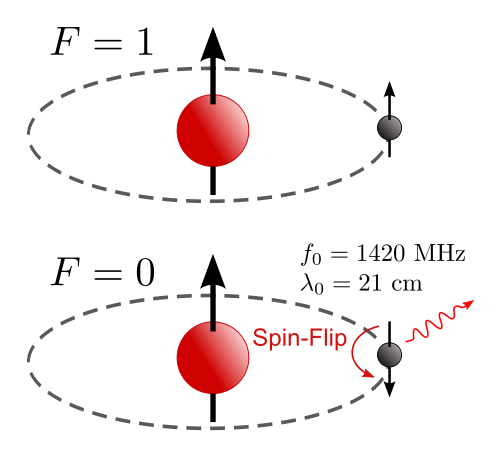
\includegraphics[width=4in]{chap0_intro/500px-Hydrogen-SpinFlip.svg.png}
	\caption[Diagram of the two Hydrogen ground states resulting from hyperfine splitting.]{Typical visualization of the two Hydrogen ground states resulting from the hyperfine splitting \citep{HydrogenSpinFlipGraphic}, where $F$ is the total angular momentum of the system, and the transition between the two states results in emission of a 21\,cm photon.}
	\label{fig:HydrogenSpinFlipGraphic}
\end{figure}

Finally, at higher order, the coupling of the proton and electron spins splits all states into those where the electron and proton spins are parallel, and those where they are antiparallel, as in Fig. \ref{fig:HydrogenSpinFlipGraphic}. The energy difference is much smaller than the differences between the $n=1,2,3$ states, and corresponds to emission or absorption of a low frequency radio photon with wavelength 21\,cm. In the upper (lower) state the spins are parallel (anti-parallel). Note that this disagrees with classical intuition, as when the spins are parallel, the magnetic dipole moments are antiparallel, and just as two antialigned magnets tend to attract, this state should actually have \textit{lower} energy. 

In response, is often remarked simply that quantum mechanics sometimes makes counterintuitive predictions, though \citet{griffiths82} argues that there is a more intuitive way to understand the situation. He observes that Fig. \ref{fig:HydrogenSpinFlipGraphic} misleadingly suggests that the electron is displaced from the proton, when in fact its spherical wavefunction encompasses it, and thus it is more correct to picture their magnetic moments as tiny current loops in the $xy$ plane (perpendicular to the proton spin). If both spins are aligned, then the current loops flow in opposite directions, and thus repel just like parallel wires with opposite currents, explaining which this is the higher energy state.

Lastly, note that in the upper state when the spins point in the same direction, the quantization of $z$ angular momentum makes this actually a spin triplet state, so there are three upper states and one lower state.

\subsection{21cm emission from the Dark Ages and Epoch of Reionization}

In this section I review theoretical calculacions of the observed 21\,cm brightness temperature of a neutral cloud in the intergalactic medium (IGM) during the Epoch of Reionization (EOR), mainly following \citet{PritchardLoebReview}, but filling in many missing details and background information where helpful. 

\subsubsection{Microscopic radiative transfer using Einstein A and B coefficients}

The Hydrogen atom is not a simple quantum mechanical system, and even less so taking into account fine and hyperfine structure, but fortunately in the cool, dilute intergalactic medium, the problem simplifies greatly. Essentially all hydrogen atoms are in the ground state at temperatures  $T<<10\text{eV}/k_B\sim10^5$K, which is always the case before the EOR when gas temperatures are $10-100$\,K, and after the EOR when they are $100-1000$\,K \citep{FurlanettoReview}. Thus only the hyperfine states are allowed, and we may regard such atoms at two level systems with an energy spacing of $\Delta E=hc/\lambda\approx6\mu$\,eV, where $\lambda=21$\,cm, and there is a three-fold degeneracy of the upper state. The four states are roughly equally populated as $T>>\Delta E/k_B =0.06$K, giving number densities of excited ($n=2$) and ground ($n=1$) state atoms as $n_2=\frac{3}{4}n_H$, and $n_1=\frac{1}{4}n_H$, where $n_H$ is the overall density of hydrogen atoms. Note that this $n=1,2$ indexes only the two hyperfine states, it is not the general $n$ used above to index all the energy levels of hydrogen. Lastly, note that the spontaneous emission lifetime of the upper excited state is roughly $10^7$\,years.

Before considering radiative transfer through the universe of 21\,cm emission from a hydrogen cloud at high redshift, we first comment on the different parts of this non-thermodynamic equilibrium problem, and present the Einstein A and B coefficients we will use to treat them. The three temperatures in this problem are: (1) the hydrogen gas temperature, encodinge the root mean square velocities of the particles; (2), the spin temperature, defined as the temperature of an ensemble of two level atoms having the same ratio of excited to ground state atoms as our system; and (3) the temperature of the cosmic microwave background, a blackbody radiation field which backlights our neutral hydrogen clouds during the EOR. 

Our task is to calculate the emergent intensity through an HI cloud with optical depth $\tau$ backlit by the CMB. From standard radiative transfer theory, the answer is $I_\nu=I_0e^{-\tau}+S_\nu(1-e^{-\tau})$, however because our three temperatures are not the same, the source function $S_\nu\equiv j_\nu/\alpha_\nu$ does not in general equal a planck (i.e., blackbody) function\footnote{The planck function is given by $B_\nu(T)\propto\nu^3/(e^{h\nu/kT}-1)$} and we thus require a microscopic description of the radiation field using the Einstein A and B coefficients.

Consider again our two level atom with number densities $n_2$ and $n_1$ in the excited and ground states, respectively. The Einstein coefficients are defined by:
\begin{eqnarray}
\text{\# spontaneous emissions per volume per time}&=&An_2 \nonumber\\
\text{\# stimulated emissions per volume per time}&=&B_{21}n_2u_\nu \nonumber\\
\text{\# absorptions per volume per time}&=&B_{12}n_1u_\nu 
\end{eqnarray}
where $u_\nu$ is the energy density per frequency of the radiation field. Note that $A$ has units of $\text{s}^{-1}$, and the $B$'s have units of $\text{s}^{-1}(\text{energy density per frequency})^{-1}$. We can construct the unit of energy density per frequency as $h\nu/(c/\nu)^3/\nu$, thus on purely dimensional grounds we expect $A\approx B (h\nu^3/c^3)$, which is the correct relation from atomic physics up to a factor of $8\pi$. Einstein showed that $g_1B_{12}=g_2B_{21}$ (where in our case $g_1=1$, $g_2=3$) regardless of whether the atoms are in thermal equilibrium with the radiation field.

Before calculating the radiation source function, let us look at the radiative transfer equation to understand how to treat stimulated emission,
\begin{equation}
\frac{dI_\nu}{ds}=j_\nu-\alpha_\nu I_\nu
\end{equation}
where $I_\nu$ is the specific intensity, with units of energy per area per solid angle per frequency per time. As the stimulated emission rate is proportional to the radiation density it makes sense to think of it contributing \textit{negatively} to the absorption coefficient. So the emission coefficient is due solely to spontaneous emission, and has units of energy per volume per time per solid angle per frequency. Integrating over the spectral line, the energy emitted per volume per time per solid angle is:
\begin{equation}
\int j_\nu d\nu=\frac{1}{4\pi}h\nu n_2 A
\end{equation}
If we introduce a line shape $\phi(\nu-\nu_0)$ with $\int\phi(\nu-\nu_0)=1$, where $\nu_0$ is the center frequency of the spectral line, then we have:
\begin{equation}
\boxed{j_\nu=\frac{h\nu_0 n_2A\phi(\nu-\nu_0)}{4\pi}}
\end{equation}

Now consider a beam with intensity $I_\nu$ passing through the atoms. The energy density in the beam is $u_\nu=I_\nu/c$, so the energy absorbed from the beam per volume per time is $\int d\nu\int d\Omega\alpha_\nu I_\nu$, which can also be expressed as $\int d\nu h\nu_0\phi(\nu-\nu_0)(n_1B_{12}-n_2B_{21})I_\nu/c$, which gives:
\begin{equation}
\boxed{\alpha_\nu=\frac{h\nu_0\phi(\nu-\nu_0)(n_1B_{12}-n_2B_{21})}{c}}
\end{equation}

Then the source function is
\begin{equation}
\boxed{S_\nu=\frac{4}{4\pi}\frac{ n_2A}{n_1B_{12}-n_2B_{21}}}
\end{equation}
which is valid even if the atoms are not in thermodynamic equilibrium with the radiation field. 

\subsubsection{Brightness temperature of an HI cloud in the EOR}

Now let us put the pieces of this calculation together and relate them to the observed emergent intensity of the CMB shining through an HI cloud during the EOR. As above, considering a radiation field with intensity $I_0$ behind a cloud of Hydrogen with optical depth $\tau$, the emergent intensity is $I_\nu=I_0e^{-\tau}+S_\nu(1-e^{-\tau})$. Cosmological redshift reduces the observed energy flux by $(1+z)$, and then reformulating the equation in terms of brightness temperatures and assuming $\tau<<1$ (because this is a very weak transition) gives
\begin{equation}
\delta T=\frac{T_s-T_\gamma(z)}{1+z}\tau 
\end{equation}
where $T_s$ is the brightness temperature of 21\,cm radiation from the gas, equal to the spin temperature of the gas\footnote{We can prove that the spin temperature equals the brightness temperature of the gas noting that $S_\nu=j_\nu/\alpha_\nu\propto A n_2/(n_1B_{12}-n_2B_{21})\propto\nu^3n_2/(3n_1-n_2/n_1)\approx\nu^2 T_s$, which is the rayleigh jeans relation with the spin temperature instead of the typical gas temperature. Note that we have used  $A\propto\nu^3B$ and $n_2/n_1\equiv3e^{-h\nu/kT_s}\approx3(1-h\nu/kT_s)$}. Now we just need the optical depth through the cloud with size $ds$.

\begin{equation}
\tau=\int\alpha ds=\int\frac{h\nu}{c}\phi(\Delta\nu)(n_1B_{12}-n_2B_{21})ds
\end{equation}
Then using $g_1B_{12}=g_2B_{21}$, $g_2/g_1=3$, and $n_2/n_1=3e^{-h\nu/kT_s}$ gives

\begin{equation}
\tau=\int\frac{h\nu}{c}\phi(\Delta\nu)\frac{n_H}{4}B_{12}(1-e^{-h\nu/kT_s})ds
\end{equation}
using $n_H=n_1/4$, given that $T_s>>h\nu/k=0.1$K. Recall that $B$ has units of $A$ divided by energy density per frequency, giving $A\sim Bh\nu^3/c^3$, and to be precise there is an $8\pi$ here. Also taylor expand the exponential:

\begin{equation}
\tau=\phi(\Delta\nu)\frac{n_H}{4}\frac{Ac^2}{8\pi\nu}\frac{h}{kT_s}\Delta s
\end{equation}
Now use that photons travel on geodesics so we may replace $\Delta s=a(t)\Delta r$ by $c\Delta t=c\Delta z/(1+z)H(z)$, and also use that the line is doppler broadened by $\Delta\nu/\nu=v/c=H(z)\Delta s/c$, with $\phi(\Delta\nu)=1/\Delta \nu$, giving:

\begin{equation}
\tau=\frac{n_H}{4}\frac{Ac^2}{\nu}\frac{h}{8\pi kT}\frac{c}{H(z)\nu}
\end{equation}

\begin{equation}
\tau=\frac{T_s-T_\gamma(z)}{1+z}\frac{\Omega_b\rho_c(1+z)^3}{4}\frac{Ac^2}{8\pi\nu}\frac{h}{kT_s}\frac{c}{H_0\sqrt{\Omega_m}(1+z)^{3/2}\nu}
\end{equation}

\begin{eqnarray}
\delta T&=&\sqrt{1+z}\left(1-\frac{T_\gamma(z)}{T_s}\right)\frac{\Omega_b}{4}\frac{3H_0}{8\pi Gm_p}\frac{h}{8\pi k}\frac{c}  {\sqrt{\Omega_m}}\left(\frac{c^2A}{\nu^2}\right)\\
&=&10\text{mK}\left(\frac{1+z}{10}\right)^{1/2}\left(1-\frac{T_\gamma(z)}{T_s}\right) 
\end{eqnarray}

again assuming $T_s>>T_\gamma$, which is the case during reionization. This derivation gives a sense of the magnitude of the differential 21\,cm brightness temperature from during reionization, which is seen to be of order tens of mK. However the exact distribution of 21\,cm emission seen in the sky depends on the density, temperature, and ionization fields. During reionization, the ionization field has the greatest influence on the 21\,cm brightness. Simulations suggest that as the first stars form, they blow out ionized bubbles around their galaxies, and the bubbles eventually merge and ionize the whole volume of the universe, save extreme overdensities in clusters. Fig. \ref{fig:mcquinneorsims} shows four different simulations of the ionization field (columns) over as a function of time (rows) during reionization. Determining which of these models, which vary parameters such as the masses and numbers of the galaxies which dominate the ionizing photon flux, is a goal of 21\,cm cosmology.

\begin{figure}
	\centering
	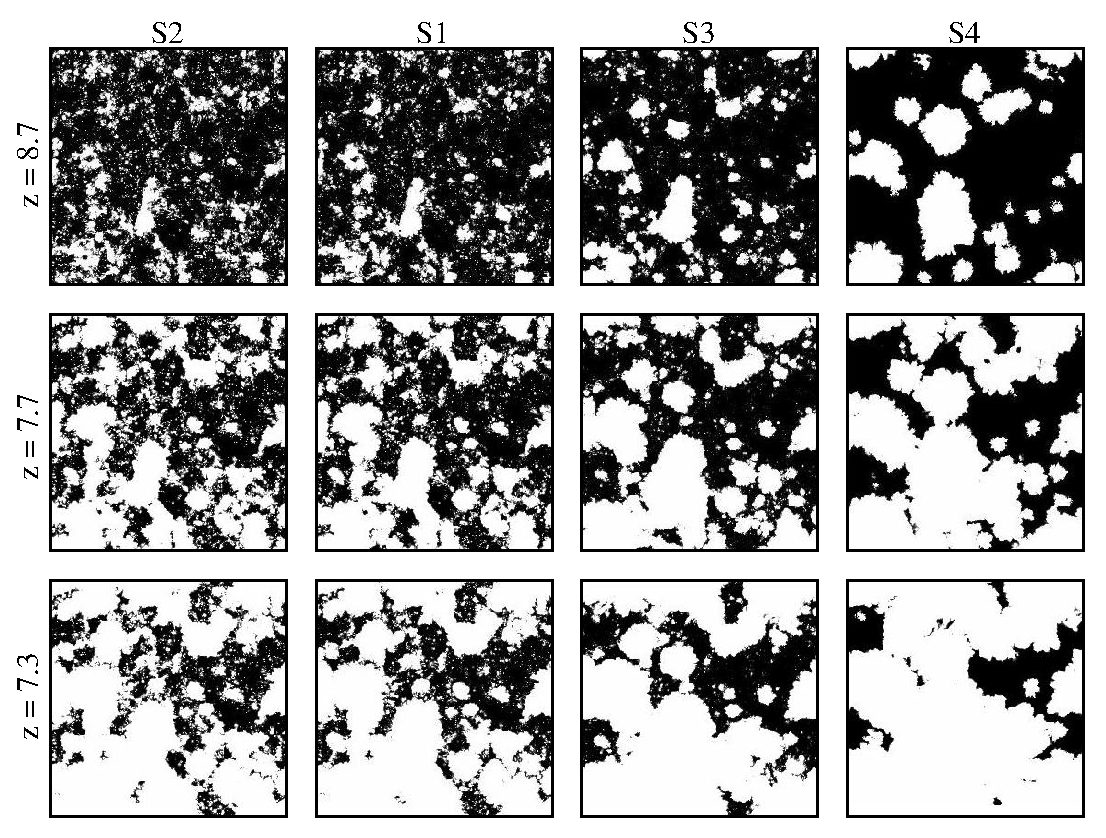
\includegraphics[width=7in]{chap0_intro/mcquinn_ionized_region_sims.eps}
	\caption[aoeuaoeu]{aeuoaoeu. Reproduced from \citet{McQuinn06}}
	\label{fig:mcquinneorsims}
\end{figure}



\subsection{Evolution of the global 21\,cm signal}

In this section we seek a sense the magnitude of the mean 21\,cm signal over cosmic time. Indeed as we saw, the brightness temperature of the 21cm signal is determined by the spin temperature, which is affected by three processes: collisional coupling with atoms and free electrons which couple the gas kinetic temperature to the spin temperature, radiative coupling to the CMB, and Ly$\alpha$-induced spin-flips via an excited state. 

As the universe evolves, the relative importance of each of these processes changes, and the spin temperature evolves accordingly. Fig. \ref{fig:pritchardloebtemperatures} shows the gas, spin, and CMB temperatures (top), the ionized fraction (center), and the differential 21\,cm brightness temperature (i.e., the 21\,cm spin temperature relative to the CMB (bottom) as a function of redshift. Three different reionization models, giving different spin and differential brightness temperature histories are presented. At $1100>z>200$ (A), the universe is dense enough so that collisional coupling between atoms and residual free electrons holds $T_\text{gas}\approx T_\gamma=T_s$, so the relative 21\,cm brightness temperature is close to zero. Then over $200>z>50$ the gas cools adiabatically, implying\footnote{Adiabatic cooling implies $PV^\gamma=$const, where $\gamma=c_p/c_v=1+1/c_v$. For a monotonic ideal gas, the specific heat at constant volume is given by $c_v=3/2$. Note also that $TV^{\gamma-1}=$const, which gives $T\sim (1+z)^2$} $T\sim (1+z)^2$. The spin temperature thus cools a factor of $1/(1+z)$ faster than the CMB, so the differential brightness temperature becomes negative (B). Note that the gas is cooling below the CMB temperature, but the gas temperature is still coupled to the spin temperature. At these high redshifts, structure is still largely linear, so that the brightness temperature traces the matter density field without corrupting \textit{gastrophysics}\footnote{Gastrophysics is a neologism refering to the astrophysics (i.e., non-cosmological) effects on the 21\,cm signal due especially to non-linear galaxy formation and feedback effects which are challenging to model.} 

\begin{figure}
	\centering
	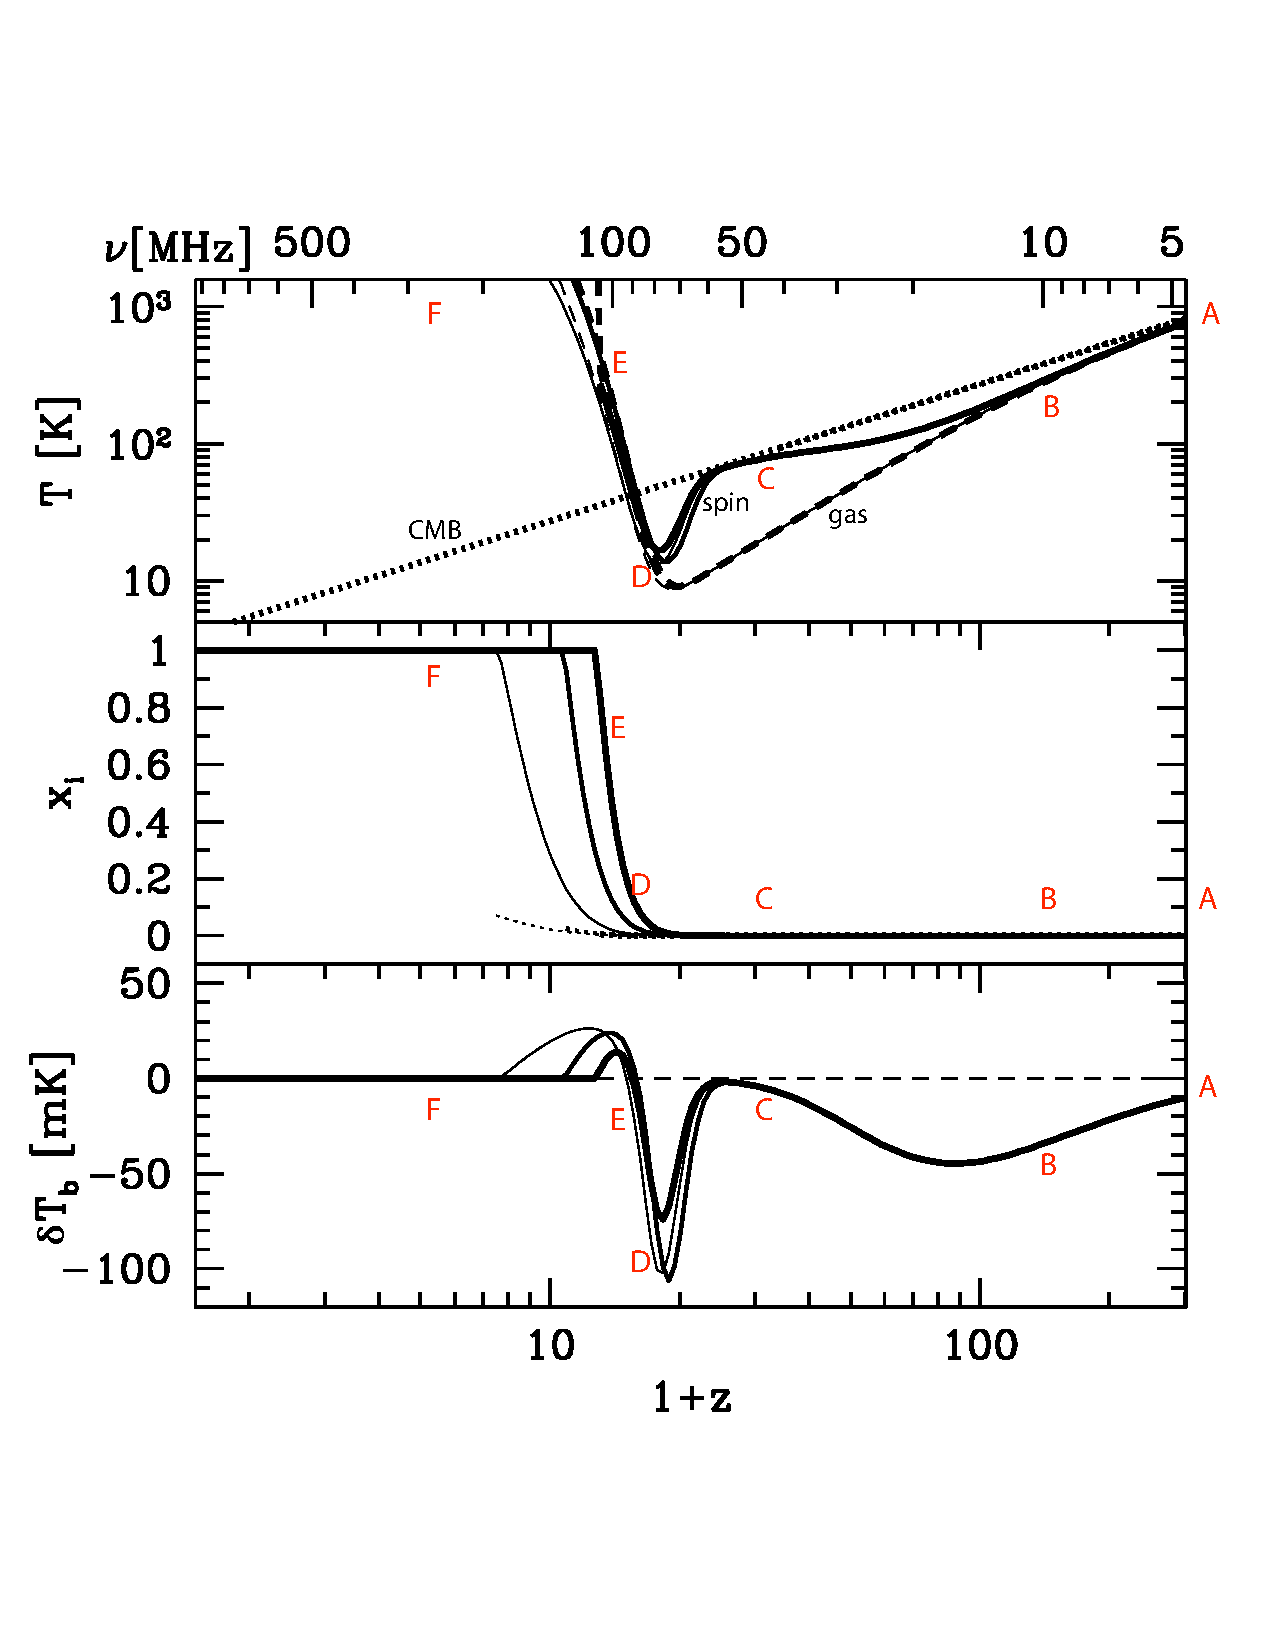
\includegraphics[width=7in]{chap0_intro/pritchard_and_loeb_temperatures_annotated.pdf}
	\caption[aoeuaoeu]{aeuoaoeu. Reproduced from \citet{PritchardLoebReview}}
	\label{fig:pritchardloebtemperatures}
\end{figure}

From here on, the exact sequence of events becomes quite uncertain. It is thought that as the universe continues to expand, the gas becomes too dilute for collisions to couple the gas and spin temperatures, and the spin temperature falls back into equilibrium with the CMB, reducing the differential brightness temperature towards zero (C). When the first sources form and begin to emit ionizing radiation, the Ly$\alpha$-induced spin flops mentioned above couple the spin temperature back to the gas temperature, which at this point is much colder than the CMB (D). In quick succession, heating of the IGM from this radiation becomes significant, raising the 21\,cm signal over the CMB temperature (E), until the bulk of the universe becomes ionized and there are no further large neutral regions to emit 21\,cm radiation (F).

\section{Measuring the 21\,cm signal with radio interferometers}

\subsection{The basics of radio interferometry}

A radio interferometer is an array of separate antennas whose outputs are correlated with each other, and combined to form an image. It is ofter cheaper and easier to use such a ``synthetic aperture'' to resolution and collecting area than to simply build ever bigger single dish antennas, especially given advances in computing over the past decades permitting real time correlation of hundreds of antennas. In this section I will review how we get from the individual antenna outputs to a sky image for a simple 1D array viewing a 1D sky.

\begin{figure}[h]
    \centering
    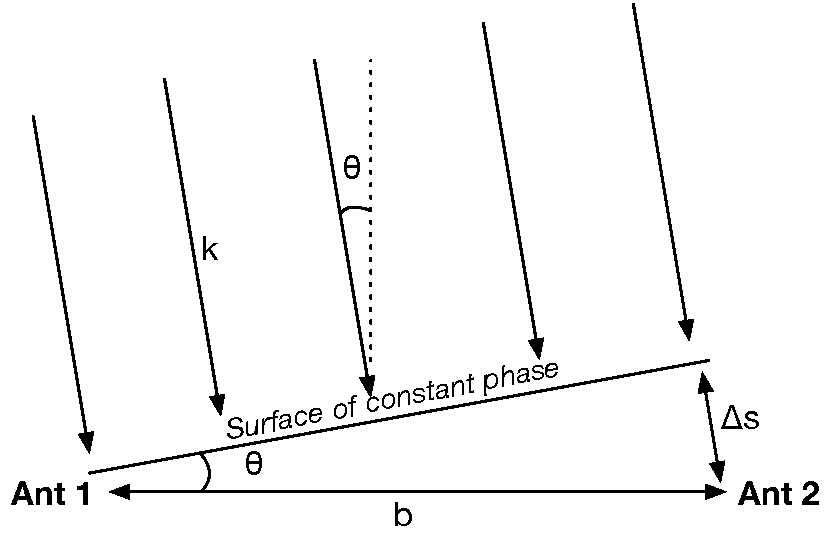
\includegraphics[width=0.95\textwidth]{chap0_intro/radio_interferometer_diagram.pdf}
    \caption[Diagram of a two element radio interferometer]{A single baseline (i.e., pair of antennas) displaced by $b$ on the ground receive radiation from a distant source at an angle $\theta$ from zenith. The source is distant enough that its surfaces of constant phase are planes which are orthogonal to $\vec{k}$, the wavevector of the radiation. The radiation arriving at Antenna 1 accumulates extra phase due to the path length difference $\Delta s$ compared to that arriving at Antenna 2.}
    \label{fig:radiointerferometerdiagram}
\end{figure}

Consider first a pair of antennas (termed a \textit{baseline}) on the ground separated by distance $b$. Radiation arrives from a distant source at an angle $\theta$ from zenith. Observe (Fig. \ref{fig:radiointerferometerdiagram}) that after the surface of constant phase reaches the first antenna, must it propagate an extra distance $\Delta s$ before reaching Antenna 2, equaling an extra phase of $\vec{k}\cdot \vec{b}=2\pi\Delta s/\lambda=2\pi\sin b/\lambda$. Then the time averaged cross correlation between the voltages measured at antenna 1 and 2, known as the visibility $V_{12}$, is
\begin{equation}
	V_{12}\equiv\langle V_1(t)V_2^*(t)\rangle=\langle(V_0^* e^{i\omega t})(V_0e^{-i(\omega t-2\pi\sin u)})\rangle \approx e^{2\pi i b\theta/\lambda}
\end{equation}
where we have used the small angle approximation, and we have switched to measuring the baseline length in units of wavelengths $u\equiv b/\lambda$. We can see that $u$ and $\theta$ are fourier dual variables. If we can measure the visibility at many different baseline lengths, then we can grid them in $u$ space and take the fourier transform to get their representation in the $\theta$ space, which is simply the sky image.

Real world interferometers have non-uniform and incomplete sampling in $u$ space, encoded by a sampling function $S(u)$. We may view this function as a sum of delta functions located at all the sampled $u$ values: $S(u)=\sum_{i,j}\delta(u_i-u_j)$, where $i,j$ index the antennas. Multiplying the true visibility function $V(u)$ by this sampling function, then fourier transforming, is equivalent (by the convolution theorem) to convolving the true sky image by the fourier transform of the sampling function, known as the synthesized beam. This is known as the \textit{dirty image}. Unlike in optical astronomy where the point spread function is close to a gaussian or an Airy function, the synthesized beam is generally non-compact with significant sidelobes due to sparse baseline sampling.  

The strategy is typically to distribute the antennas pseudo randomly to achieve as many different baselines as possible, calculate the dirty image, then use an iterative procedure known as CLEAN \citep{hogbomclean} to incrementally deconvolve the synthesized beam from the true sky image under the assumption that the true sky is predominantly a collection of isolated point sources. The statistics of the resulting \textit{clean image} are difficult to quantify as CLEAN is a non-linear algorithm, but in practice it is found to work quite well and is indispensable to characterizing the compact radio sources between us and the EOR signal (i.e., foregrounds).

\subsection{From image cubes to power spectra}

First generation experiments lack the sensitivity to directly image 21\,cm emission from the EOR, aiming instead to statistical detections of the signal through different methods of combining many pixels, each with SNR<1, into a significant detection. The most prominent of these methods is estimation of the power spectrum.

To understand how cosmological power spectrum measurements are made, let us first consider the space the interferometer measurements live in. Interferometer measurements consist of cross correlations, or visibilities, at different frequencies. We have shown in the previous section that each visibility is a measurement of a different sky fourier mode $(u,v)$, which are dual coordinates to $(\theta_x,\theta_y)$. However, each frequency corresponds to a different cosmological redshift, and thus, distance from us. Interferometric visibilities thus live in an awkward mixed fourier space: To study foregrounds, we must fourier transform along $u$ and $v$ to reach 3D image space, but to make power spectrum measurements, we must transform along $f$ to reach 3D fourier space. This is illustrated in Fig. \ref{fig:ifospace}, where we denote the fourier dual to $f$ as $\eta$, termed \textit{delay}.

\begin{figure}[h]
    \centering
    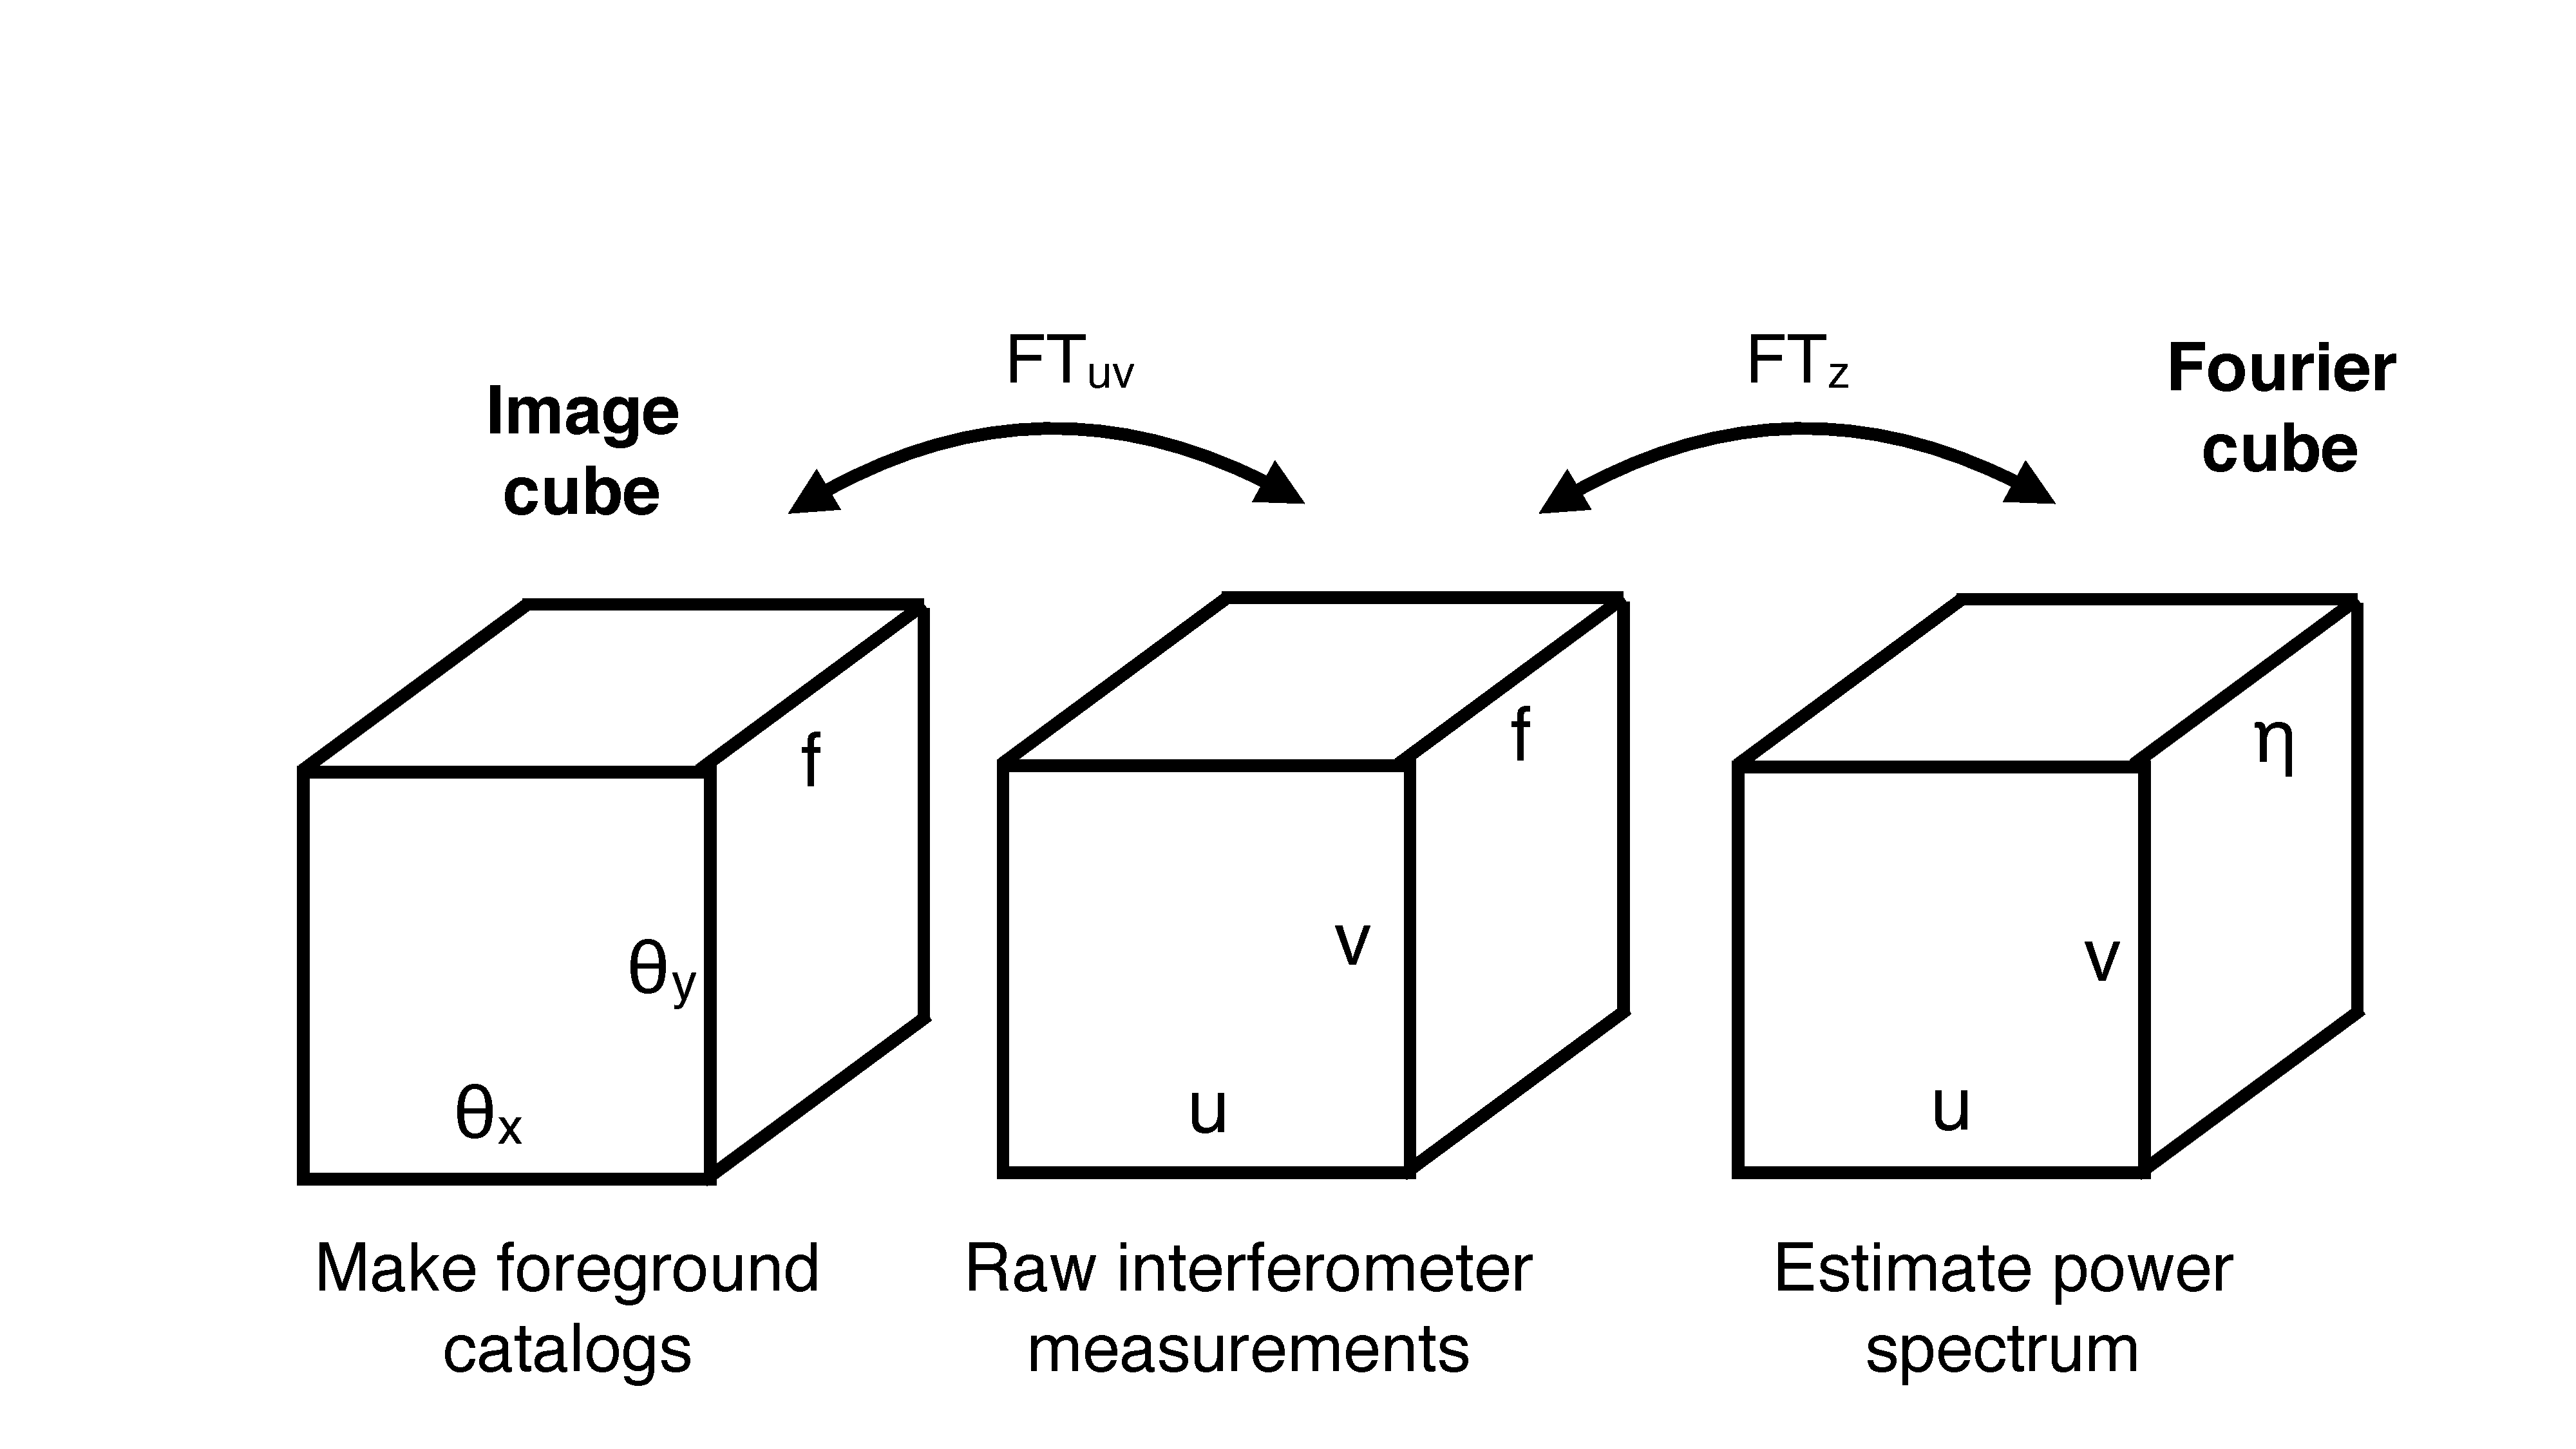
\includegraphics[width=1\textwidth]{chap0_intro/ifo_space.pdf}
    \caption[Representation of the relation between image space, fourier space, and interferometer space]{aoeuaoeu}
    \label{fig:ifospace}
\end{figure}

We seek to estimate the spatial power spectrum of 21\,cm emission in comoving units, that is, as a function of wave number $k$ with units of inverse comoving distance. We must first transform $u$ and $v$ to $k_x$ and $k_y$. For brevity, consider only the $x$ dimension. $u$ is defined by the fourier factor $e^{2\pi i u\theta}$, which we must match with $k_x$, defined by $e^{ik_x x}$, where $x$ is the comoving distance transverse to the line of sight. Setting their exponents equal and using $x=D\theta$, where $D$ is the comoving distance to the redshift of interest, we find.

\begin{eqnarray}
	k_x=\frac{2\pi u}{D} \\ 
	k_y=\frac{2\pi v}{D} \\ 
\end{eqnarray}

To relate $k_z$ to $\eta$, we must first match the exponents in $e^{i k_z x_\parallel}$ and $e^{i\omega \eta}$, where $x_\parallel$ is the comoving distance along the line of sight\footnote{Unfortunately we can't refer to this as $z$ because it's taken by the cosmological redshift.} and $\omega=2\pi f$ gives the observation frequency. Matching these, and using that $d x_\parallel/df=cf_0/H(z)f^2$, we find

\begin{equation}
	k_z=\frac{2\pi\eta f_0 H(z)}{c(1+z)^2}
\end{equation}

\begin{figure}[h]
    \centering
    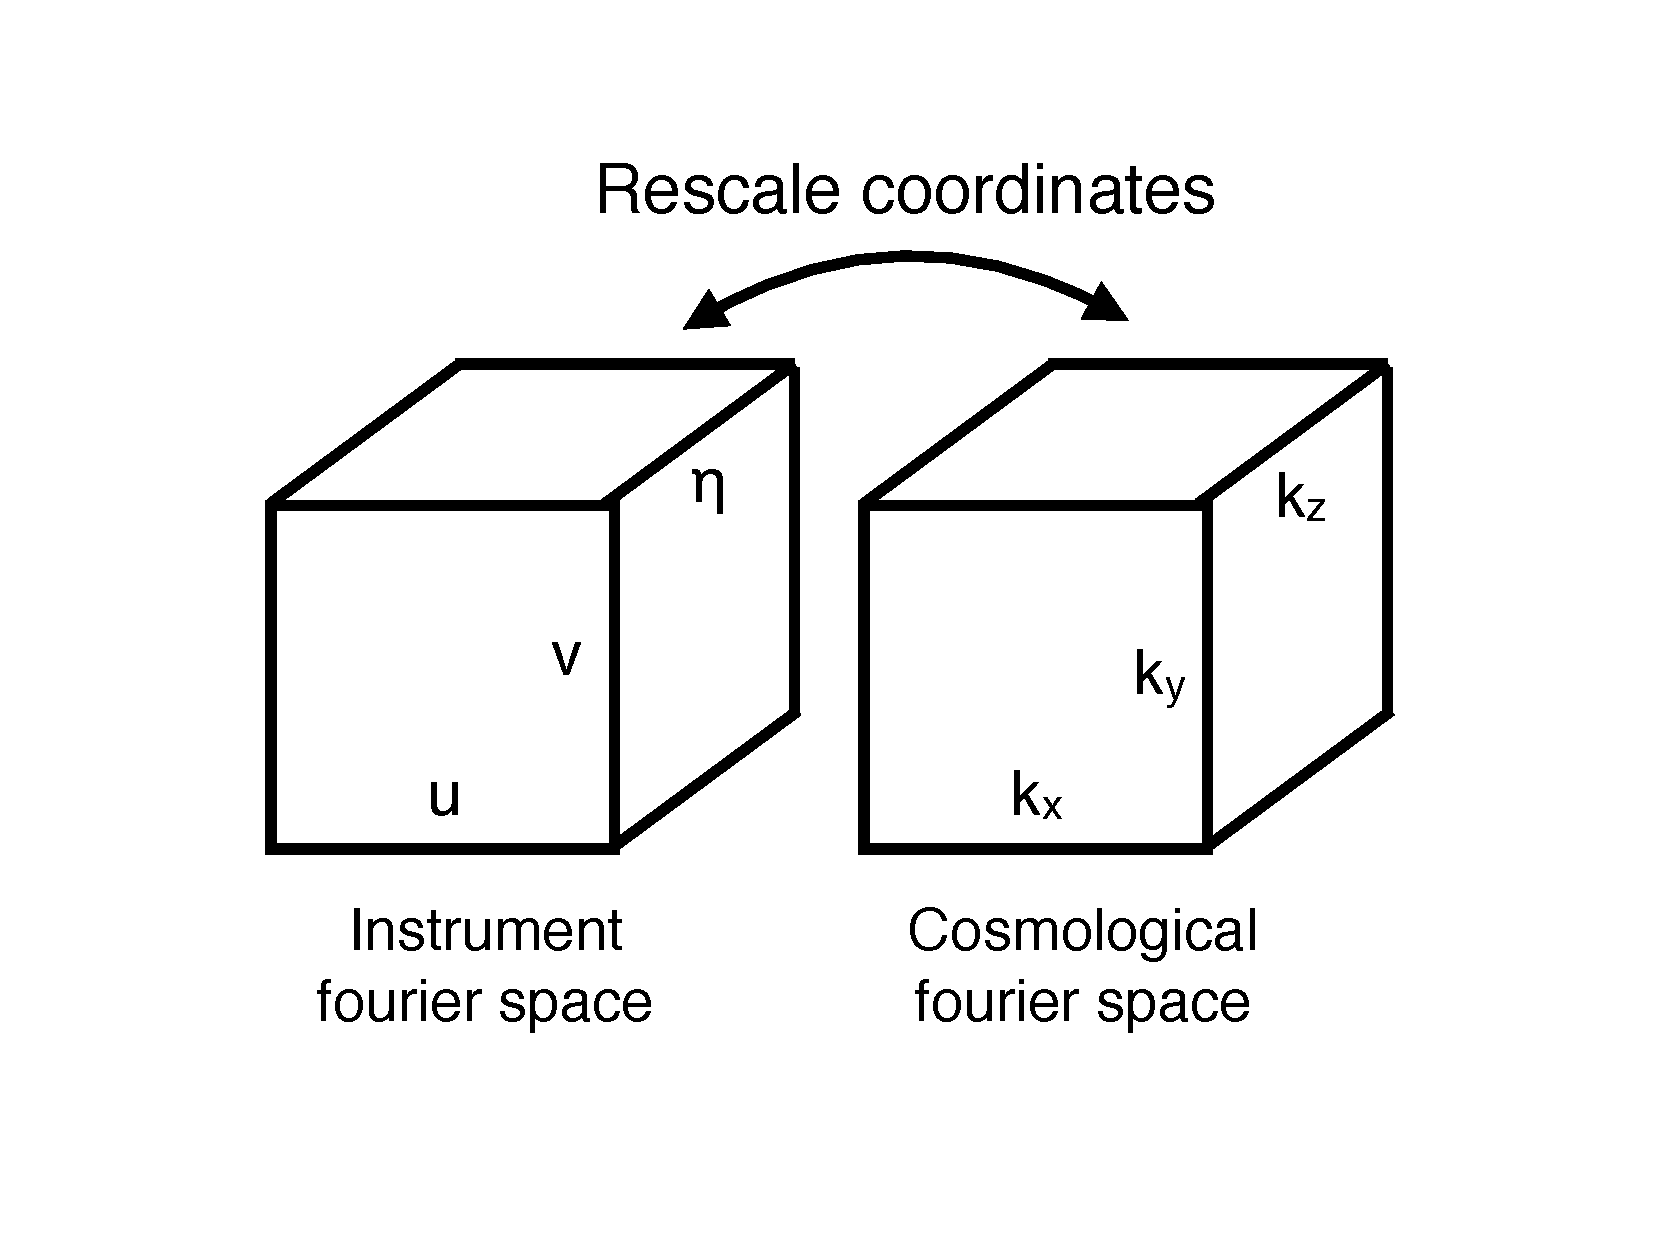
\includegraphics[width=0.9\textwidth]{chap0_intro/ifo_space_cosmo.pdf}
    \caption[Representation of the relation between image space, fourier space, and interferometer space]{aoeuaoeu}
    \label{fig:ifospacecosmo}
\end{figure}

A last note is that to characterize foregrounds, we often combine $k_x$ and $k_y$ together to plot the \textit{cylindrically} binned power spectrum as a function of $k_\perp\equiv(k_x^2+k_y^2)^{1/2}$ and $k_\parallel\equiv k_z$.

%optimal quadratic power spectrum estimators, essentially, generalized FT with arbitrary weighting



\subsection{Sensitivity challenges}
\label{sec:sensitivity}

The two major challenges to observing redshifted 21\,cm emission from the dark ages and EOR are sensitivity and foregrounds. Interferometers at low frequencies are sky noise dominated, meaning that the diffuse galactic synchrotron dominates the received antenna power, and thus, the visibility noise. However it is so diffuse, and thus, so compact in $uv$ space, that its contribution to the visibility means is negligible. See Appendix A for a full discussion of sky noise. Our concern here is that in the coolest parts of the sky, at high galactic latitudes, galactic synchrotron has brightness temperatures of $\sim200$\,K \citep{Tsysmemo}. The cosmological global signal is at the tens of mK level, and simulations suggest that individual fourier modes are far smaller, at the few mK level. 

Let us get a sense for the sensitivity challenge with a rough calculation. I show in Appendix A that the noise $\sigma_V$ on visibility $V_{ij}$ is given by $V_{ii}/\sqrt{Bt}$ where $V_{ii}$ is the autocorrelation, $B$ is the bandwidth, and $t$ is the observation time. Measuring the sky in brightness temperature units, the autocorrelation is given by $V_{ii}=\int T(\hat\theta)d\Omega\sim T_\text{sky}\Omega$, where $\Omega=\lambda^2/A$ is the solid angle of the beam main lobe. Comparing this brightness temperature noise with the expected few mK cosmological visibilities, gives roughly 100 hours for a 5$\sigma$ detection. Note that this is not the total length of time observing. As the earth rotates, baselines are projected and rotated to different parts of the $uv$ plane. Over several hours of observing, many baselines enter and exit the $uv$ cell in question, and in general many more than 100 hours of observing is needed to achieve 100 hours in each cell. 

However, as alluded to above, we don't need 5$\sigma$ detections in every $uv$ cell to make a detection of the power spectrum of 21\,cm emission. Consider a simple case where we neglect the frequency dimension. Let raw visibilities have noise $\sigma_V$, and each $uv$ cell is the average of $N_\text{vis.per.cell}$ of them. Then the power spectrum is is estimated by averaging the power over the $N_\text{cells}$ cells with similar $\sqrt{u^2+v^2}$ magnitude. The noise on the mean visibility $\bar{V}$ in each cell is $\sigma_V/\sqrt{N_\text{vis.per.cell}}$, and the noise $\sigma_{\bar V^2}$ is $\sqrt{\langle\bar V^4\rangle-\langle\bar V^2\rangle^2}\sim\sigma_V/\sqrt{N_\text{vis.per.cell}}$, which is reduced by $1/\sqrt{N\text{cells}}$ when spherically binning. So we find 

\begin{equation}
	\sigma_P\propto\frac{\sigma_V^2}{N_\text{vis.per.cell}\sqrt{N_\text{cells}}}
\end{equation}

Thus we see that there are two kinds of averaging which reduce the level of thermal noise in the power spectrum: \textit{coherent} averaging (by a factor of $1/N_\text{vis.per.cell}$) within individual $\vec{k}$ modes, and \textit{incoherent} averaging (by a factor of $1/\sqrt{N_\text{cells}}$) of power over different $\vec{k}$ modes falling into the same spherical $k$ bin. In the first case, we average different measurements of the same true value but with different noise, whereas in the second case, we average different realizations of the true spherical bandpower $k$. Were there no thermal noise on our measurements, the first average would do nothing, but the second would help to reduce sample variance noise. 

So we see that sensitivity of a real interferometer is set by the amount of coherent and incoherent binning of thermal noise, due to the 200\,K diffuse galactic synchrotron emission.  \citet{beardsley13} predict a $7\sigma$ detection of the power spectrum with the Murchison Widefield Array after 450\,hours, and \citet{PoberNextGen} predict a 3--7$\sigma$ detection after 1080\,hours, depending on foreground properties. In contrast to the MWA, whose antennas are distributed pseudo randomly to maximize the number of $uv$ modes sampled, PAPER's antennas are placed on a grid. Thus very few $uv$ modes are sampled, which makes imaging extremely challenging, but from a power spectrum point of view, they have optimized for coherent averaging at the expense of incoherent averaging. \citet{PoberNextGen} thus predict comparable sensitivities to the MWA despite their substantially smaller antennas. HERA builds on both sets of lessons learned, employing ultimately 350 14\,m dishes on a grid, and should yield tens of $\sigma$ detection \citet{neben16b,ewallwice16,nithya16,PoberNextGen}. 

\subsection{Foreground challenges}

While the diffuse synchrotron emission in our galaxy generates the noise on our measurements, compact extragalactic radio sources between us and the EOR generate a bias. We term these these sources \text{foregrounds}, though the rest of the astronomy community terms them \textit{science}. Over the 100-200\,MHz band corresponding to redshifted 21\,cm emission from the EOR, foreground emission is sourced by radio synchrotron generated by relativistic electrons gyrating around galactic magnetic field lines. I derive in Appendix \ref{chap:synchrotron} that synchrotron emission has a power law spectrum with $I\sim\nu^{-0.75}$.

The smooth spectral structure of foregrounds is key to distinguishing them from the blotchy reionizing universe (Fig. \ref{fig:mcquinneorsims}). A line of sight through the EOR passes through some neutral regions and some ionized regions, making the overall 21\,cm emission from the neutral regions, all at slightly different redshifts, appear spectrally very unsmooth. Early work proposed removing smooth structure  from every line of sight through the cube separately, subtracting splines, low order polynomials, or eigenforegrounds \citep{Judd08, paper1, paper2,xiaomin,LOFAR2,Harker,Jelic08,MoralesBowmanHewittFGsub}. However, simulations \citep{Dattapowerspec}, early theory \citep{VedanthamWedge,MoralesPSShapes,CathWedge,nithya13}, and early data analyses have shown that this is not the whole story. The frequency-dependent $uv$ sampling of interferometer baselines causes spectrally smooth foreground power to leak into higher $k_\parallel$ modes. Said differently, as a function of frequency, each baseline samples a different fourier mode of the sky, and that effect cannot be perfectly removed by simply gridding the baseline to a different $uv$ cell at different frequencies. Longer baselines move through $uv$ space faster with frequency, and this linear dependence manifests after gridding many baselines to $k_\perp,k_\parallel$ space as wedge-shaped region containing the preponderance of foreground power. 

Work to understand this leakage is ongoing. \citet{AdrianWedge1,AdrianWedge2} show that it introduces not only a bias to the power spectrum but error correlations as well. It also manifests differently \citep{pober13} in the approximate power spectra computed using the per-baseline technique of \citet{parsonsandbacker,parsons12b} than using the image-based power spectra of \citep{beardsley16,dillonneben,X13}. 

Knowing this, two basic approaches to foreground removed have been discussed in the literature: foreground avoidance and foreground subtraction. The former consists of simply excluding modes in the wedge from power spectrum estimation, albeit at a non-negligible sensitivity hit, while the latter requires subtraction of 99.99\% of foreground intensity. Both are challenging, and neither has yet resulted in an EOR detection, but new experiments such as the under-construction HERA \citep{neben16,ewallwice16,nithya16,deboer16} and the next generation SKA \citep{ska,ska1,ska2,ska3} should achieve highly significant detections in even the most pessimistic foreground cases. 

\subsection{Large N--small D arrays and their challenges}

In this section I will introduce the class of experiments being conducted to observe spatial fluctuations in 21\,cm emission from the EOR, and outline the experimental challenges they pose. As discussed in Sec. \ref{sec:sensitivity}, detection of 21\,cm from the EOR demands hundreds of hour integrations on arrays with hundreds of antennas. Even so, arrays such as MWA, PAPER, LOFAR, and now HERA are targeting only a statistical detection of the emission, that is, detection of a smooth power spectrum rather than high SNR images of ionizing bubbles. The latter demands even more sensitivity, and must await the Square Kilometer Array, an array planning literally nearly a square kilometer of antenna collecting area on the ground. 

With these enormous demands on collecting area, cost of a handful of enormous dishes would be prohibitive, especially as it would need to steer around the sky to avoid foregrounds and the galactic plane. Typical radio interferometers over the past decades have consisted of a few or a few dozen steerable dishes such as the Very Large Array, the Giant Meterwave Radio Telescope, the Westerbork Synthesis Radio Telescope, and now the Atacama Large Millimeter Array. 

The 21\,cm arrays listed above instead represent a new generation of low frequency radio interferometry made possible by advances in large scale digital signal processing, computing, and storage. Indeed PAPER was so named after Don Backer's famous aphorism that what was required to detect the EOR was ``paperclips and supercomputers.'' At meter-wavelengths, antenna fabrication precision is largely irrelevant, and pointing is done far more cheaply with beamforming (ie, by placing smaller antennas into phased arrays) than with steerable dishes. 

Effectively eschewing hardware investment for software investment is not without its challenges, though, in fact many traditional techniques of radio astronomy are proving insufficient and the community is grappling with how to improve them. Work on better antenna measurement, gain and phase calibration, radio frequency interference flagging, source cataloging, and quality control is ongoing in order to make cosmological 21\,cm observations a reality, and this thesis is part of that larger effort. Over the remainder of this section, I will outline the specific challenges that large N--small D arrays are posing experimentally, and what is being done to address them.

\begin{itemize}
	\item \textbf{Antenna measurement} 
	\item \textbf{Gain and phase calibration} 
	\item \textbf{Quality control} 
	\item \textbf{Source cataloging} 
\end{itemize}



big data / quality control (cite beardsley)
\citep{beardsley16}

primary beam measurements, wide field problem, no clean fields

gain calibration: sky models are imperfect at low frequencies, cite Aaron EW's recent calibration paper, an Braun, cite danny's precision+accuracy paper
\citep{jacobs2013,braun2013,ewallwice16b}

a slightly bigger antenna element has an advantage (HERA)
\citep{deboer16}

%\section{Roadmap of this thesis}


%\section{Completing the picture with cross correlations}
%
%\subsection{examples of successful cross correlation results}
%Tzu-Ching's result \citep{Chang2010,Masui2013}
%
%\subsection{what could be learned from IR cross correlation}
%more about the sources: pop2 vs pop3
%topology of reionization, anticorrelation scale shows bubble size increasing over time
%
%\citep{Heneka2016}
%\citep{Fernandez2014,Silva2012,Mao2014,Lidz2008,Gong2014,Fernandez2013}
%
